\begin{center}
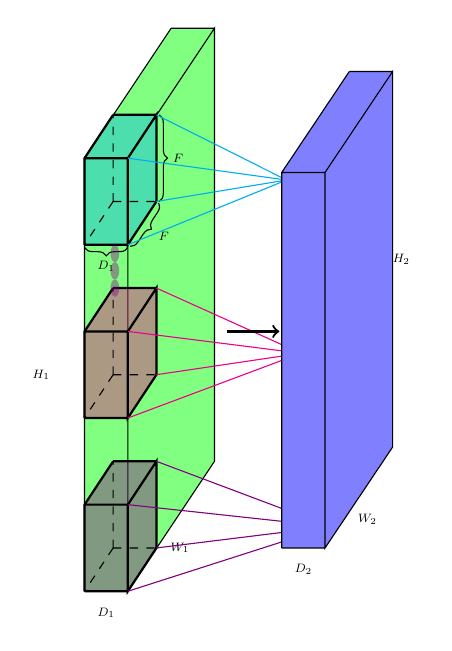
\begin{tikzpicture}[scale=.55, transform shape]
\def\h{10}
\def\w{2}
\def\d{3}
\coordinate (A) at (0,0);
\coordinate (B) at (0,\h);
\coordinate (C) at (\w,\h+\d);
\coordinate (D) at (\w,\d);

\coordinate (A1) at (0+1,0);
\coordinate (B1) at (0+1,\h);
\coordinate (C1) at (\w+1,\h+\d);
\coordinate (D1) at (\w+1,\d);


\fill [draw=none, fill=green!50] (A) -- (B) -- (C) -- (C1) -- (D1) -- (A1) -- cycle; 

\draw (A) -- (B) -- (C) (A) -- (A1) (B) -- (B1) (C) -- (C1) (A1) -- (B1) -- (C1) -- (D1) -- cycle;

\onslide<3->{
\draw [color=white,decorate,decoration={brace,amplitude=10pt,raise=1pt},xshift=0pt,yshift=0pt] (A) -- (B) node [black,midway,xshift=-1cm] {\footnotesize $H_1$};
}
\onslide<4->{
\draw [color=white,decorate,decoration={brace,amplitude=3pt,raise=1pt},xshift=-4pt,yshift=0pt] (A1) -- (A) node [black,midway,yshift=-0.5cm] {\footnotesize $D_1$};
}
\onslide<2->{
\draw [color=white, decorate,decoration={brace,amplitude=10pt,mirror,raise=1pt},xshift=0pt,yshift=0pt] (A1) -- (D1) node [black,midway,xshift=0.2cm,yshift=-0.5cm] {\footnotesize $W_1$};
}

\def\ha{2}
\def\wa{0.66}
\def\sa{1}
\def\wb{0.33}%shift
\def\sb{0.5}%shift
\def\hc{0.66}%next layer box
\def\wc{0.22}%next layer box size
\def\sc{0.33}
\def\xm{4} %distance of next box
\def\xmv{0.22}
\def\ymv{1}
\def\wid{1}
%\def\mycolor{red}

\edef\y{8}
\edef\x{0}


		%feature map 1, points
		\coordinate (A4) at (0+\x*\wb+\xm+\xmv,0+\y+\x*\sb+\ymv);
		\coordinate (B4) at (0+\x*\wb+\xm+\xmv,\hc+\y+\x*\sb+\ymv);
		\coordinate (C4) at (\wc+\x*\wb+\xm+\xmv,\hc+\sc+\y+\x*\sb+\ymv);
		\coordinate (D4) at (\wc+\x*\wb+\xm+\xmv,\sc+\y+\x*\sb+\ymv);
		%\edef\xta{\wc*0.5+\x*\wb+\xm+\xmv}
		%\edef\yta{\y+\x*\sb+\ymv+\hc*0.5+\sc*0.5}		


		

%\foreach \mycolor [count=\xi from 1] [count=\yi from 2] in {cyan,magenta,orange,violet}{				
		\onslide<6->{
		\edef\mycolor{cyan}
		\edef\myval{0.3333}		
		\edef\y{8}
		%\edef\x{\xi}
		%layer1 feature map coordinates
		\coordinate (A6) at (0+\xm+\xmv+\myval,0+\ymv);
		\coordinate (B6) at (0+\xm+\xmv+\myval,\h-\sc);
		\coordinate (C6) at (\w+\xm-\xmv+\myval,\h+\d-\ymv);
		\coordinate (D6) at (\w+\xm-\xmv+\myval,\d+\sc);		
		
		\coordinate (A2) at (0+\x*\wb,0+\y+\x*\sb);
		\coordinate (B2) at (0+\x*\wb,\ha+\y+\x*\sb);
		\coordinate (C2) at (\wa+\x*\wb,\ha+\sa+\y+\x*\sb);
		\coordinate (D2) at (\wa+\x*\wb,\sa+\y+\x*\sb);
		
		\coordinate (A3) at (0+1+\x*\wb,0+\y+\x*\sb);
		\coordinate (B3) at (0+1+\x*\wb,\ha+\y+\x*\sb);
		\coordinate (C3) at (\wa+1+\x*\wb,\ha+\sa+\y+\x*\sb);
		\coordinate (D3) at (\wa+1+\x*\wb,\sa+\y+\x*\sb);		
		
		
		\coordinate (ABCD4) at (\wc*0.5+\x*\wb+\xm+\xmv+\myval,\y+\x*\sb+\ymv+\hc*0.5+\sc*0.5);

		\fill [draw=none, fill=\mycolor, fill opacity=0.4] (A2) -- (B2) -- (C2) -- (C3) -- (D3) -- (A3) -- cycle; 
			
		\draw[thick] (A2) -- (B2) -- (C2) (A2) -- (A3) (B2) -- (B3) (C2) -- (C3) (A3) -- (B3) -- (C3) -- (D3) -- cycle;
		\draw[dashed] (D2) -- (A2) (D2) -- (C2) (D2) -- (D3);
	\onslide<8->{
\draw [decorate,decoration={brace,amplitude=3pt,raise=1pt},xshift=0pt,yshift=0pt] (C3) -- (D3) node [black,midway,xshift=0.5cm] {\footnotesize $F$};

\draw [decorate,decoration={brace,amplitude=3pt,raise=1pt},xshift=-4pt,yshift=0pt] (A3) -- (A2) node [black,midway,yshift=-0.5cm] {\footnotesize $D_1$};

\draw [decorate,decoration={brace,amplitude=3pt,mirror,raise=1pt},xshift=0pt,yshift=0pt] (A3) -- (D3) node [black,midway,xshift=0.5cm,yshift=-0.3cm] {\footnotesize $F$};		
	}
		
		\onslide<7->{
		\draw[\mycolor] (A3) -- (ABCD4) (B3) -- (ABCD4) (C3) -- (ABCD4) (D3) -- (ABCD4);
		
		\fill[\mycolor] (ABCD4) ellipse (0.1 and 0.2);
		}
		\onslide<7->{
		\fill [draw=none, fill=\mycolor] (A6) -- (B6) -- (C6) --  (D6) -- cycle;			
		}
		
		}	
		
		\onslide<7->{
		\edef\mycolor{magenta}
		\edef\myval{2*0.3333}		
		\edef\y{4}
		%\edef\x{\xi}
		%layer1 feature map coordinates
		\coordinate (A26) at (0+\xm+\xmv+\myval,0+\ymv);
		\coordinate (B26) at (0+\xm+\xmv+\myval,\h-\sc);
		\coordinate (C26) at (\w+\xm-\xmv+\myval,\h+\d-\ymv);
		\coordinate (D26) at (\w+\xm-\xmv+\myval,\d+\sc);		
		
		\coordinate (A22) at (0+\x*\wb,0+\y+\x*\sb);
		\coordinate (B22) at (0+\x*\wb,\ha+\y+\x*\sb);
		\coordinate (C22) at (\wa+\x*\wb,\ha+\sa+\y+\x*\sb);
		\coordinate (D22) at (\wa+\x*\wb,\sa+\y+\x*\sb);
		
		\coordinate (A23) at (0+1+\x*\wb,0+\y+\x*\sb);
		\coordinate (B23) at (0+1+\x*\wb,\ha+\y+\x*\sb);
		\coordinate (C23) at (\wa+1+\x*\wb,\ha+\sa+\y+\x*\sb);
		\coordinate (D23) at (\wa+1+\x*\wb,\sa+\y+\x*\sb);		
		
		
		\coordinate (ABCD24) at (\wc*0.5+\x*\wb+\xm+\xmv+\myval,\y+\x*\sb+\ymv+\hc*0.5+\sc*0.5);

		\fill [draw=none, fill=\mycolor, fill opacity=0.4] (A22) -- (B22) -- (C22) -- (C23) -- (D23) -- (A23) -- cycle; 
			
		\draw[thick] (A22) -- (B22) -- (C22) (A22) -- (A23) (B22) -- (B23) (C22) -- (C23) (A23) -- (B23) -- (C23) -- (D23) -- cycle;
		\draw[dashed] (D22) -- (A22) (D22) -- (C22) (D22) -- (D23);
		
		\onslide<7->{
		\draw[\mycolor] (A23) -- (ABCD24) (B23) -- (ABCD24) (C23) -- (ABCD24) (D23) -- (ABCD24);
		
		\fill[\mycolor] (ABCD24) ellipse (0.1 and 0.2);
		}
		\onslide<7->{
		\fill [draw=none, fill=\mycolor] (A26) -- (B26) -- (C26) --  (D26) -- cycle;			
		}	
		
		}
		
		\onslide<7->{
		\edef\mycolor{violet}		
		\fill[\mycolor,fill opacity=0.4] (0.7+\x*\wb,0+\y+\x*\sb-0.2) ellipse (0.1 and 0.2);
		\fill[\mycolor,fill opacity=0.4] (0.7+\x*\wb,0+\y+\x*\sb-0.6) ellipse (0.1 and 0.2);
		\fill[\mycolor,fill opacity=0.4] (0.7+\x*\wb,0+\y+\x*\sb-1) ellipse (0.1 and 0.2);
		}
		\onslide<7->{
		\edef\myval{4*0.3333}		
		\edef\y{0}
		%\edef\x{\xi}
		%layer1 feature map coordinates
		\coordinate (A16) at (0+\xm+\xmv+\myval,0+\ymv);
		\coordinate (B16) at (0+\xm+\xmv+\myval,\h-\sc);
		\coordinate (C16) at (\w+\xm-\xmv+\myval,\h+\d-\ymv);
		\coordinate (D16) at (\w+\xm-\xmv+\myval,\d+\sc);		
		
		\coordinate (A12) at (0+\x*\wb,0+\y+\x*\sb);
		\coordinate (B12) at (0+\x*\wb,\ha+\y+\x*\sb);
		\coordinate (C12) at (\wa+\x*\wb,\ha+\sa+\y+\x*\sb);
		\coordinate (D12) at (\wa+\x*\wb,\sa+\y+\x*\sb);
		
		\coordinate (A13) at (0+1+\x*\wb,0+\y+\x*\sb);
		\coordinate (B13) at (0+1+\x*\wb,\ha+\y+\x*\sb);
		\coordinate (C13) at (\wa+1+\x*\wb,\ha+\sa+\y+\x*\sb);
		\coordinate (D13) at (\wa+1+\x*\wb,\sa+\y+\x*\sb);		
		
		
		\coordinate (ABCD14) at (\wc*0.5+\x*\wb+\xm+\xmv+\myval,\y+\x*\sb+\ymv+\hc*0.5+\sc*0.5);

		\fill [draw=none, fill=\mycolor, fill opacity=0.4] (A12) -- (B12) -- (C12) -- (C13) -- (D13) -- (A13) -- cycle; 
			
		\draw[thick] (A12) -- (B12) -- (C12) (A12) -- (A13) (B12) -- (B13) (C12) -- (C13) (A13) -- (B13) -- (C13) -- (D13) -- cycle;
		\draw[dashed] (D12) -- (A12) (D12) -- (C12) (D12) -- (D13);
		
		%\draw [decorate,decoration={brace,amplitude=12pt,raise=1pt},xshift=0pt,yshift=0pt] (A3) -- (B13) node [black,midway,xshift=1.4cm] {\footnotesize $K$ filters};		
		
		}
		\onslide<7->{
		\draw[\mycolor] (A13) -- (ABCD14) (B13) -- (ABCD14) (C13) -- (ABCD14) (D13) -- (ABCD14);
		
		\fill[\mycolor] (ABCD14) ellipse (0.1 and 0.2);
		}
		\onslide<7->{
		\fill [draw=none, fill=\mycolor] (A16) -- (B16) -- (C16) --  (D16) -- cycle;	
		}
		
		
		\onslide<9->{
			\fill [draw=none, fill=blue!50] (A6) -- (B6) -- (C6) -- (C16) -- (D16) -- (A16) -- cycle;			
			\draw (A6) -- (B6) -- (C6) (A6) -- (A16) (B6) -- (B16) (C6) -- (C16) (A16) -- (B16) -- (C16) -- (D16) -- cycle;
			
		\draw[thick,->] (3.3,6) -- (4.5,6);
\draw [color=white, decorate,decoration={brace,amplitude=10pt,raise=1pt},xshift=0pt,yshift=0pt] (C16) -- (D16) node [black,midway,xshift=0.2cm] {\footnotesize $H_2$};

\draw [color=white, decorate,decoration={brace,amplitude=3pt,raise=1pt},xshift=-4pt,yshift=0pt] (A16) -- (A6) node [black,midway,yshift=-0.5cm] {\footnotesize $D_2$};

\draw [color=white, decorate,decoration={brace,amplitude=10pt,mirror,raise=1pt},xshift=0pt,yshift=0pt] (A16) -- (D16) node [black,midway,xshift=0.2cm,yshift=-0.5cm] {\footnotesize $W_2$};
		}
%}


\end{tikzpicture}
\end{center}